% \input{\pSections "sec-results"}

\section{Results}

%     %     %     %     %     %     %     %     %
\subsection{Fidelity of Approximation}
\begin{frame}{Fourier Transform Visualizations at 16 MHz}
    \centering
    \begin{tabular}{ccc}
        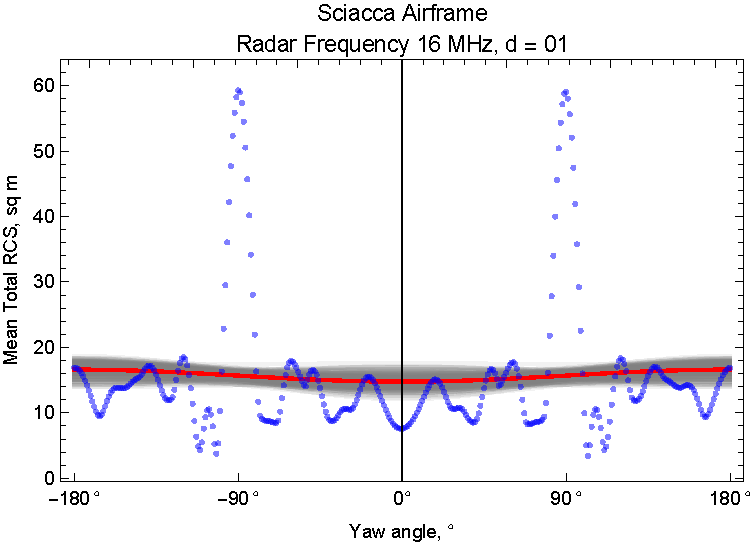
\includegraphics[ width = 0.3\textwidth ]{ \pLocalGraphics/wh-fourier-16Mhz-d01.pdf } & 
        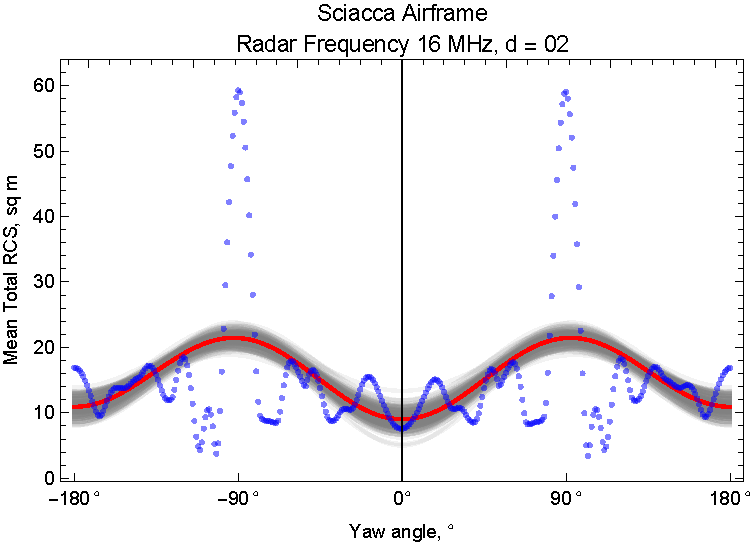
\includegraphics[ width = 0.3\textwidth ]{ \pLocalGraphics/wh-fourier-16Mhz-d02.pdf } & 
        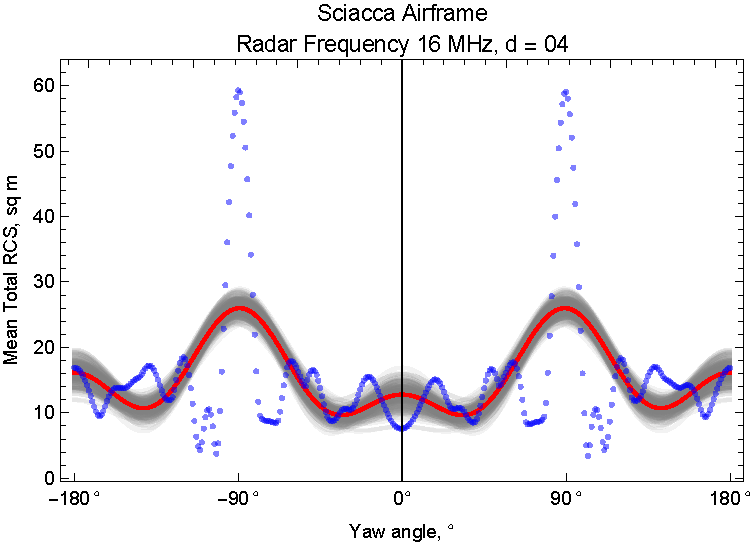
\includegraphics[ width = 0.3\textwidth ]{ \pLocalGraphics/wh-fourier-16Mhz-d04.pdf } \\
        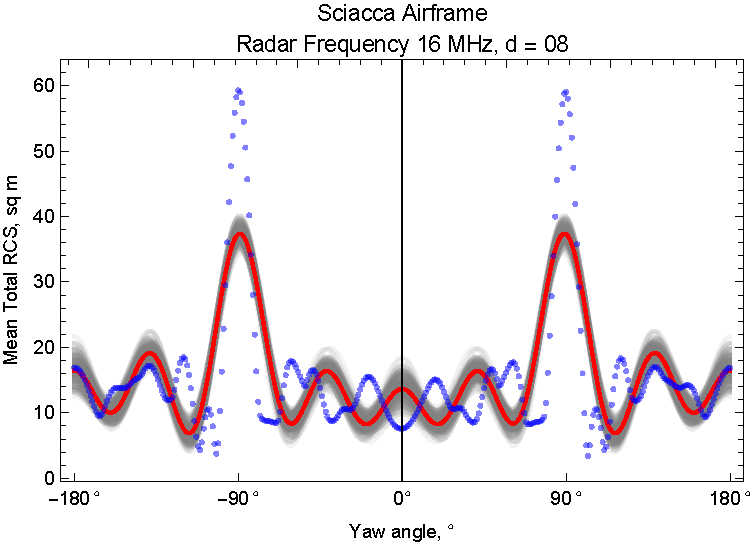
\includegraphics[ width = 0.3\textwidth ]{ \pLocalGraphics/wh-fourier-16Mhz-d08.pdf } & 
        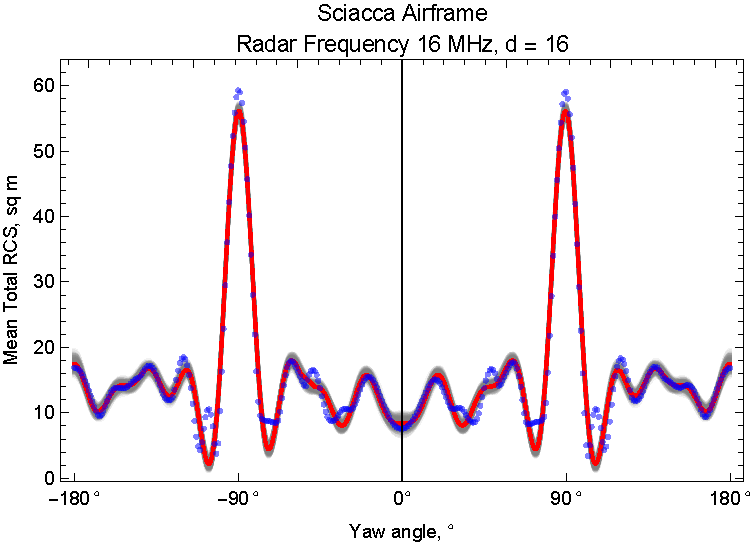
\includegraphics[ width = 0.3\textwidth ]{ \pLocalGraphics/wh-fourier-16Mhz-d16.pdf } & 
        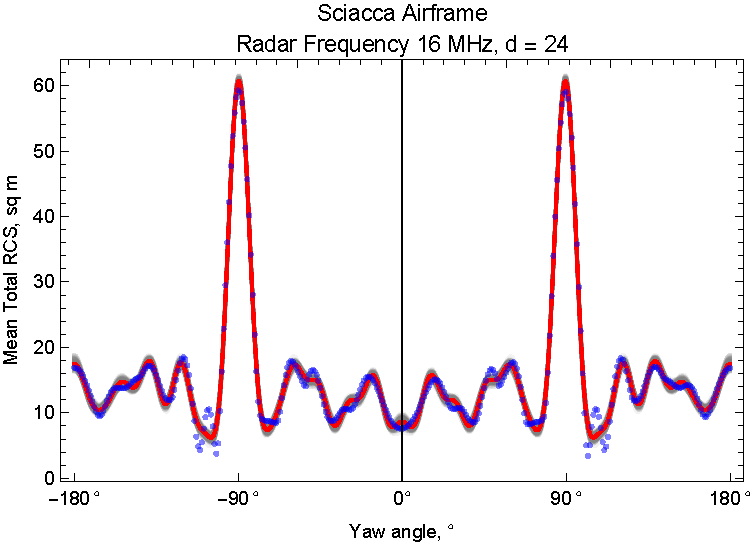
\includegraphics[ width = 0.3\textwidth ]{ \pLocalGraphics/wh-fourier-16Mhz-d24.pdf } \\
    \end{tabular}
    \vspace{0.0em}
    %\caption{Visualizations of the Fourier Transform at 16 MHz for Different Parameters.}
    \begin{block}{\centering \footnotesize Note}
         \footnotesize {\textcolor{blue}{Blue:} Data \hspace{1em} \textcolor{red}{Red:} Approximation \hspace{1em} \textcolor{gray}{Gray:} Error}
    \end{block}
    \label{tab:fidelity}
\end{frame}

\begin{frame}{Fourier Transform Visualizations at 16 MHz}
    \small
    \begin{itemize}
        \item \textcolor{blue}{Approximation Order (\(d\)):} 
              The number of terms in the Fourier approximation increases as \(d = 1, 2, 4, 8, 16, 24\).
        \item \textcolor{blue}{Low-Order Approximations:} 
              Approximations with smaller \(d\) (e.g., \(d = 1, 2, 4\)) fail to capture fine structures, leading to significant residual error.
        \item \textcolor{blue}{Higher-Order Approximations:} 
              As \(d\) grows, the approximation better resolves finer features, and the error (gray) shrinks significantly, especially at smooth regions.
        \item \textcolor{blue}{Error Behavior:} 
              The error decreases non-uniformly—large errors persist near abrupt changes or peaks due to Gibbs phenomena, but smooth regions converge faster.
        \item \textcolor{blue}{Key Insight:} 
              Fourier approximations demonstrate trade-offs: computational complexity increases with \(d\), but fidelity improves.
        \item \textcolor{blue}{General Notes:}
              \begin{itemize}
                  \item Fourier series represent functions as sums of sines and cosines.
                  \item Low-frequency terms approximate broad trends; high-frequency terms capture fine details.
                  \item Convergence is faster for smooth functions but slower for discontinuities or sharp changes.
                  \item Increasing the number of terms improves fidelity but can introduce numerical artifacts if not handled carefully.
              \end{itemize}
    \end{itemize}
\end{frame}

\begin{frame}{Fourier Transform Visualizations at 16 MHz}
    \small
    \begin{itemize}
        \item \textcolor{blue}{Approximation Order (\(d\)):} 
              The number of terms in the Fourier approximation increases as \(d = 1, 2, 4, 8, 16, 24\).
        \item \textcolor{blue}{Low-Order Approximations:} 
              Approximations with smaller \(d\) (e.g., \(d = 1, 2, 4\)) fail to capture fine structures, leading to significant residual error.
        \item \textcolor{blue}{Higher-Order Approximations:} 
              As \(d\) grows, the approximation better resolves finer features, and the error (gray) shrinks significantly, especially at smooth regions.
        \item \textcolor{blue}{Error Behavior:} 
              The error decreases non-uniformly—large errors persist near abrupt changes or peaks due to Gibbs phenomena, but smooth regions converge faster.
    \end{itemize}
\end{frame}

\begin{frame}{Fourier Transform Visualizations at 16 MHz}
    \small
    \begin{itemize}
        \item \textcolor{blue}{Key Insight:} 
              Fourier approximations demonstrate trade-offs: fidelity improves with \(d\), as does computational cost.
        \item \textcolor{blue}{General Notes:}
              \begin{itemize}
                  \item Fourier series resolve functions as sums of sines and cosines.
                  \item Low-frequency terms: broad trends; high-frequency:e fine details.
                  \item Convergence is faster for smooth functions but slower for discontinuities or sharp changes.
                  \item More terms improves fidelity, but can introduce numerical artifacts.
              \end{itemize}
    \end{itemize}
\end{frame}


%     %     %     %     %     %     %     %     %
\subsection{Linear Independence}
	
%     %     %     %     %     %     %     %     %
\subsection{Quality of Fit}

\endinput  %  ==  ==  ==  ==  ==  ==  ==  ==  ==
